% DOC SETTINGS ===================================
\documentclass{article}
\usepackage[utf8]{inputenc}
\usepackage{fancyhdr}
\pagestyle{fancy}
\usepackage{geometry}
 \geometry{
 a4paper,
 total={170mm,257mm},
 left=20mm,
 top=25mm,
 }
\fancyheadoffset{0mm}
\lhead{ECE2024 Formula Sheet}
\rhead{Kavin Thirukonda 2020}
\usepackage{steinmetz}
\usepackage{mathtools}  
\mathtoolsset{showonlyrefs} 

% DOC SETTINGS ===================================
\begin{document}
% Exam 1 ===================================
\section*{Exam One}
\newpage
% Exam 1 ===================================
% Exam 2 ===================================
\section*{Exam Two}
\subsection*{Series RLC}
\begin{equation}
\alpha = \frac{R}{2L}
\end{equation}
\begin{equation}
\omega_0 = \frac{1}{\sqrt{LC}}
\end{equation}
\begin{center}
The R used in the formula is based on the resistance seen at the terminals of the \textbf{capacitor} for $t > 0$.
    
Because in the R is in the numerator, un-damped condition occurs when $R = 0$
\end{center}

\subsection*{Parallel RLC}
\begin{equation}
\alpha = \frac{1}{2RC}
\end{equation}
\begin{equation}
\omega_0 = \frac{1}{\sqrt{LC}}
\end{equation}
\begin{center}
The R used in the formula is based on the resistance seen at the terminals of the \textbf{inductor} for $t > 0$.

Because in the R is in the denominator, un-damped condition occurs when $R = \infty$
\end{center}
\subsection*{RLC Response}
\begin{equation}
\zeta = \frac{\alpha}{\omega_0}
\end{equation}
\begin{equation}
\omega = \sqrt{\omega_0^2-\alpha^2}
\end{equation}
\begin{equation}
    s_1 = -\alpha + \sqrt{\alpha^2 - \omega_0^2}
\end{equation}
\begin{equation}
    s_2 = -\alpha - \sqrt{\alpha^2 - \omega_0^2} 
\end{equation}
\begin{center}
$\zeta$ is the \textbf{damping ratio}

$\alpha$ is the \textbf{damping coefficient}

$\omega_0$ is the \textbf{resonant frequency} 

$\omega$ is the \textbf{natural frequency/damped frequency} 

$s_1,s_2$ are the \textbf{roots of the characteristic equation} 
\end{center}
\subsubsection*{Over-Damped Response}
For $\zeta > 1$:
\begin{equation}
    x(t) = x(\infty) + K_1e^{s_1 t}+K_2e^{s_2 t}
\end{equation}
\subsubsection*{Critically-Damped Response}
For $\zeta = 1$:
\begin{equation}
     x(t) = x(\infty) + K_1e^{-\alpha t}+K_2te^{-\alpha t}
\end{equation}
\subsubsection*{Under-Damped Response}
For $\zeta < 1$:
\begin{equation}
    x(t) = x(\infty) + K_1e^{-\alpha t}cos(\omega t)+K_2e^{-\alpha t}sin(\omega t)
\end{equation}
\newpage
\subsection*{Phasors and Impedances}
\begin{center}
    for any sinusoidal function like so:
    
    $x(t) = Acos(\omega t + \phi)$
    
    An associated phasor can be written in the form ($\phi$ in \textbf{degrees}):
    
    $A \phase {\phi}$
\end{center}
\begin{center}
      Period, Frequency, and Angular Frequency:
\end{center}
\begin{equation}
    \omega = 2\pi f = \frac{2\pi}{T}
\end{equation}
\begin{equation}
    f = \frac{1}{T}
\end{equation}
\begin{center}
    \textbf{Current} leads in a \textbf{Capacitive} circuit.
    
    \textbf{Voltage} leads in a \textbf{Inductive} circuit.
\end{center}

\subsubsection*{Useful Trig Identities}
\begin{equation}
    sin(A) = cos(A - 90)
\end{equation}
\begin{equation}
    cos(A) = sin(A + 90)
\end{equation}
\begin{equation}
    e^{jA} = cos(A) + jsin(A)
\end{equation}
\begin{equation}
    rad = \frac{\pi*degrees}{180^\circ}
\end{equation}
\begin{equation}
    degrees = \frac{180^\circ * rad}{\pi}
\end{equation}
\subsubsection*{RMS}
\begin{equation}
      X_{rms} = \sqrt{\frac{1}{T}\ \int_{0}^{T} x(t)^2 \,dt }
\end{equation}
\begin{center}
    The RMS value for any sinusoidal function is:
\end{center}    
\begin{equation}
      \frac{A}{\sqrt{2}}
\end{equation}
\begin{center}    
    where A is the maximum amplitude of the function.
\end{center}
\subsubsection*{Impedances}
\begin{center}
    The impedance of an \textbf{inductor} is given as:
\end{center}
\begin{equation}
    Z_L = j\omega L
\end{equation}
\begin{center}
    The impedance of an \textbf{capacitor} is given as:
\end{center}
\begin{equation}
    Z_C = \frac{1}{j\omega C}
\end{equation}
\begin{center}
    or
\end{center}
\begin{equation}
    Z_C = \frac{-j}{\omega C}
\end{equation}
\begin{center}
    Impedances in \textbf{series} can be added:
\end{center}
\begin{equation}
    Z_{eq} = Z_1 + Z_2 + ... + Z_n
\end{equation}
\begin{center}
    Impedances in \textbf{parallel} can be flippy floppy added:
\end{center}
\begin{equation}
    Z_{eq} = [\frac{1}{Z_1} + \frac{1}{Z_2} + ... + \frac{1}{Z_n}]^{-1}
\end{equation}
\subsubsection*{Complex Power}
\begin{center}
    Average Real Power:
\end{center}
\begin{equation}
    V_{rms}I_{rms}cos(\theta_v - \theta_i)
\end{equation}
\begin{center}
    Peak Reactive Power:
\end{center}
\begin{equation}
    jV_{rms}I_{rms}sin(\theta_v - \theta_i)
\end{equation}
\subsection*{First and Second Order Filters}
\begin{center}
    The filter transfer function is defined as:
\end{center}
\begin{equation}
    H(f) = \frac{V_{out}\phase{\theta_{out}}}{V_{in}\phase{\theta_{in}}} => V_{out}\phase{\theta_{out}} = H(f)*V_{in}\phase{\theta_{in}}
\end{equation}
\begin{equation}
    f_B =  \frac{R}{2\pi L} = \frac{\alpha}{\pi}
\end{equation}
\begin{equation}
    f_B =  \frac{1}{2\pi RC} = \frac{\alpha}{\pi}
\end{equation}
\subsubsection*{First Order Low Pass}
\begin{equation}
    H(f) =  \frac{1}{1+j(\frac{f}{f_B})^2}
\end{equation}
\begin{equation}
    |H(f)| =  \frac{1}{\sqrt{1+(\frac{f}{f_B})^2}}
\end{equation}
\begin{equation}
    \phase{H(f)} =  tan^{-1}(\frac{f}{f_B})
\end{equation}
\subsubsection*{First Order High Pass}
\begin{equation}
    H(f) =  \frac{j\frac{f}{f_B}}{1+j\frac{f}{f_B}}
\end{equation}
\begin{equation}
    |H(f)| =  \frac{\frac{f}{f_B}}{\sqrt{1+(\frac{f}{f_B})^2}}
\end{equation}
\begin{equation}
    \phase{H(f)} =  90 - tan^{-1}(\frac{f}{f_B})
\end{equation}
\subsubsection*{Second Order Filters}
\begin{center}
    at the resonant frequency ($f_0$): $|Z_{C  }|=|Z_{L}|$
    
    it is the frequency at which the circuits equivalent impedance is purely resistive
\end{center}
\begin{equation}
    f_0 = \frac{1}{2\pi\sqrt{LC}}
\end{equation}
\begin{equation}
    2\pi f_0 =  \omega_0 = \frac{1}{\sqrt{LC}}
\end{equation}
\subsection*{Quality Factor}
\begin{equation}
    Q_s = 2 \zeta 
\end{equation}
\begin{center}
    When $Q_s < \frac{1}{2}$ the circuit is Overdamped.
\end{center}
\begin{center}
    When $Q_s = \frac{1}{2}$ the circuit is Critically-damped.
\end{center}
\begin{center}
    When $Q_s > \frac{1}{2}$ the circuit is Underdamped.
\end{center}
\newpage
% Exam 2 ===================================
% Exam 3 ===================================
\section*{Exam Three}
\subsection*{Op Amps}
\begin{center}
    Op amp ideal characteristics:

    No current flows \textbf{into} the input pins
    
    voltage difference \textbf{between} the pins is zero
    \vspace{5mm}
    
    a \textbf{Differentiator} circuit can be made with a capacitor in \textbf{series} with an op amp
    
    a \textbf{Integrator} circuit can be made with a capacitor in \textbf{parallel} with an op amp
\end{center}
\subsubsection*{Inverting Op-amp}
\begin{center}
    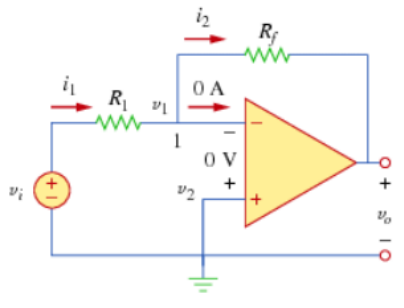
\includegraphics[width = .15\textwidth]{inverting.png}
\end{center}
\begin{equation}
    v_{out} = -\frac{R_f}{R_{in}}v_{in}
\end{equation}
\subsubsection*{Non-Inverting Op-amp}
\begin{center}
    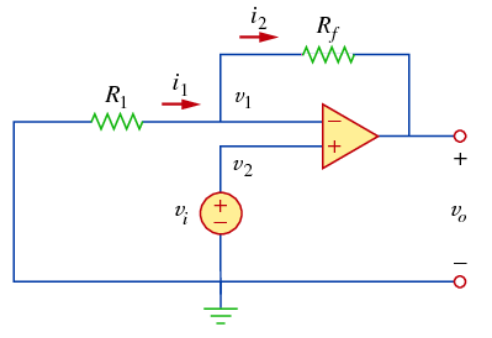
\includegraphics[width = .15\textwidth]{noninverting.png}
\end{center}
\begin{equation}
    v_{out} = (1 +\frac{R_f}{R_{in}})v_{in}
\end{equation}
\subsubsection*{Buffer}
\begin{center}
    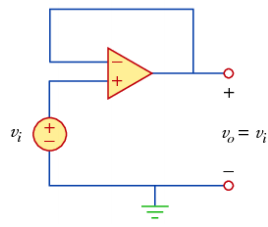
\includegraphics[width = .15\textwidth]{buffer.png}
\end{center}
\begin{equation}
    v_{out} = v_{in}
\end{equation}
\subsubsection*{Summer Op-amp}
\begin{center}
    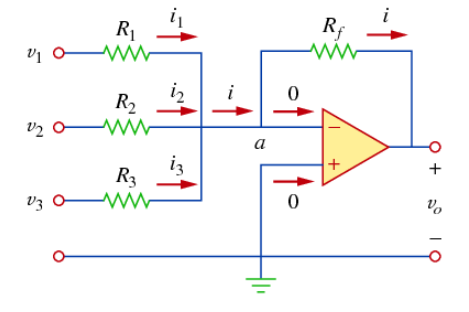
\includegraphics[width = .15\textwidth]{summer.png}
\end{center}
\begin{equation}
    v_{out} = -(\frac{R_f}{R_2}v_1 + \frac{R_f}{R_2}v_2 +\frac{R_f}{R_3}v_3)
\end{equation}
\subsubsection*{Differential Op-amp}
\begin{center}
    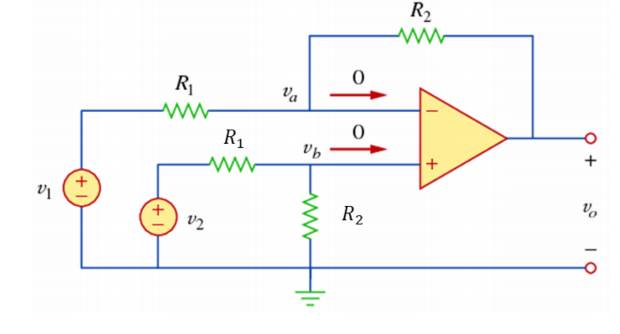
\includegraphics[width = .15\textwidth]{differential.png}
\end{center}
\begin{equation}
    v_{out} = \frac{R_2}{R_1}(v_2 - v_1)
\end{equation}
\subsection*{Active Filters}
\begin{center}
        By using the characteristics of op-amps with negative feedback the transfer functions of active filters can be found by analysing them in parts separating them where there is a buffering action.
        
        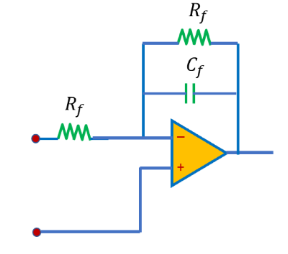
\includegraphics[width = .25\textwidth]{activeLPF.png}
        
        Above is the most basic inverting \textbf{low pass} filter.
        
        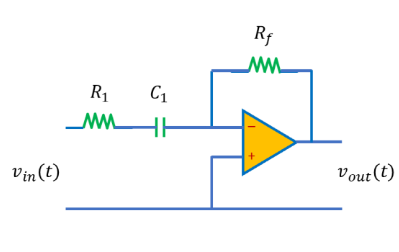
\includegraphics[width = .3\textwidth]{activeHPF.png}
        
        Above is the most basic inverting \textbf{high pass} filter.
        
        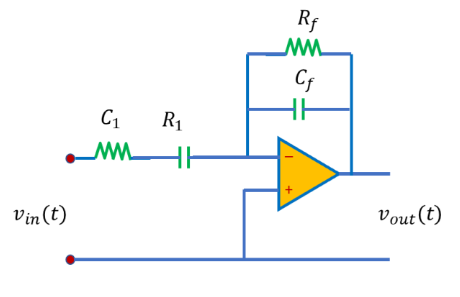
\includegraphics[width = .3\textwidth]{activeBPF.png}
        
        Above is the most basic inverting \textbf{band pass} filter.
        \vspace{3mm}
        Similar to passive filters there are many variations of filters that can be made with active filters. By doing this there are some common filter designs that are often used, the three most common are \textbf{Butterworth}, \textbf{Tshebyscheff}, \textbf{Bessel}
        
        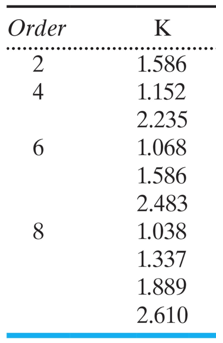
\includegraphics[width = .15\textwidth]{butterworth.png}
        
        Butterworth Polynomial Chart
        
        The chart above is required for certain calculations for designing Butterworth circuits.
\end{center}
\subsection*{Diodes}
\begin{center}
    Diode are made using doped semiconductors, the P-type doping (Phosphorus) is the Anode of the diode, and the N-type doping (Boron) is the cathode of the diode.
    \vspace{5mm}
    The forward voltage of a diode is $\phi_f = V_f \cong 0.7V$
    
    The ideal diode can be characterized with the Shockley diode equation:
\end{center}
\begin{equation}
    i_d = I_s [exp(\frac{v_d}{n V_T}) -1]
\end{equation}
\begin{center}
    $I_s$ is the \textbf{Saturation Current}
    
    $V_T$ is the \textbf{Thermal Voltage} $ \approx .026$ @ room temperature
    
    $n$ is the \textbf{Quality Factor}
\end{center}
\subsubsection*{Load-line Analysis}
\begin{center}
    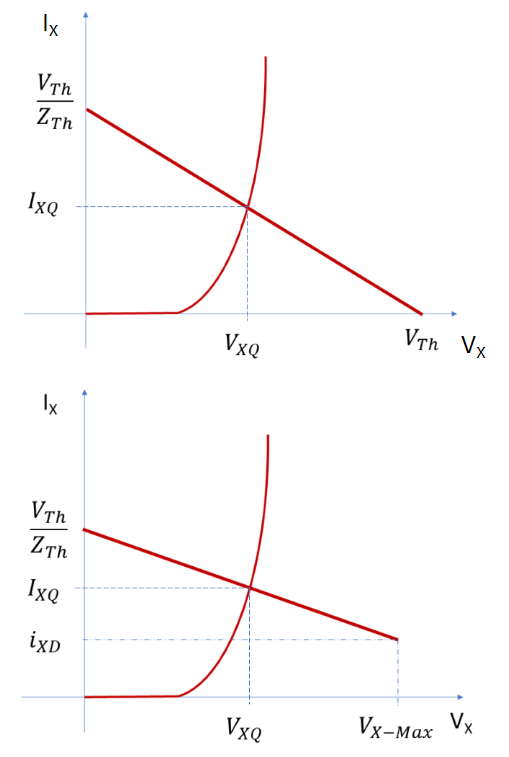
\includegraphics[width = .3\textwidth]{loadline.png}
    
    if $V_{th}$ is out of range for the plot given use the following formula:
\end{center}
\begin{equation}
    i_{XD} = \frac{V_{th} - V_{x-max}}{R_{th}}
\end{equation}
\subsubsection*{Small Signal Model}
\begin{equation}
    r_d = \frac{\Delta v_D}{\Delta i_D} \approx \frac{n V_T}{i_{D_Q}}
\end{equation}
\begin{center}
    $r_d$ is the \textbf{dynamic resistance}, it models the linearization of the circuit.
\end{center}
\newpage
\subsection*{Clippers and Clampers}
\subsubsection*{Clippers}
\begin{center}
    Clippers block AC voltages after a certain point in the waveform, this is good if a certain circuit cannot accept more than a certain voltage.
    
    To calculate the negative and positive bounds, add up the forward voltages of the diodes.
\end{center}
\subsubsection*{Clampers}
\begin{center}
    Clampers shift AC voltages up and down by a certain constant value, this is good to shift the voltage to a certain range than may be more useful for a given circuit.
    
    Similarly to clippers, to calculate the shift, just add up the forward voltages of the diodes.
\end{center}
\subsection*{BJT Basics}
\begin{center}
    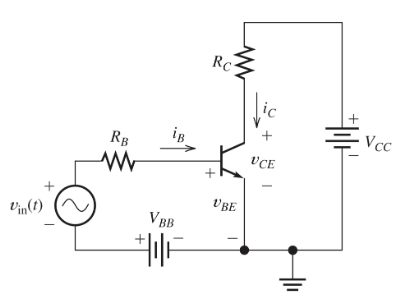
\includegraphics[width = .5 \textwidth]{basicBJT.png}
\end{center}
\begin{equation}
    \alpha = \frac{i_c}{i_e} = \frac{\beta}{1 + \beta}
\end{equation}
\begin{equation}
    \beta = \frac{i_c}{i_b} = \frac{\alpha}{1-\alpha}
\end{equation}
\begin{equation}
    i_B = i_E - i_C
\end{equation}

\begin{center}
$\beta$ is the \textbf{useful gain}
\end{center}
\subsubsection*{NPN}
\begin{center}
    Variations of the Shockley equation for the NPN BJT:
\end{center}
\begin{equation}
    i_E = I_{ES}[exp (\frac{v_{BE}}{V_t}) -1]
\end{equation}
\begin{equation}
    i_C = \alpha I_{ES}[exp (\frac{v_{BE}}{V_t}) -1]
\end{equation}
\begin{equation}
    i_B = (1 - \alpha)I_{ES}[exp (\frac{v_{BE}}{V_t}) -1]
\end{equation}
\subsubsection*{PNP}
\begin{center}
    Variations of the Shockley equation for the PNP BJT:
\end{center}
\begin{equation}
    i_E = I_{ES}[exp (\frac{-v_{BE}}{V_t}) -1]
\end{equation}
\begin{equation}
    i_C = \alpha I_{ES}[exp (\frac{-v_{BE}}{V_t}) -1]
\end{equation}
\begin{equation}
    i_B = (1 - \alpha)I_{ES}[exp (\frac{-v_{BE}}{V_t}) -1]
\end{equation}
\newpage
\subsection*{Large Signal Model for BJTs}
\begin{center}
    The Large-Signal model is used for the DC analysis of the BJT. It helps us solve problems related to the DC bias of the BJT.
    
    Instead of a single Large-Signal Model, we have 3 large-signal models, one for each of the regions of operation of the BJT, each of these models varies depending on if the BJT is a PNP or NPN.
    
    For a model to be accurate, \textbf{all} constraints of the model must be met.
\end{center}
\subsubsection*{Forward-Active}
\begin{center}
    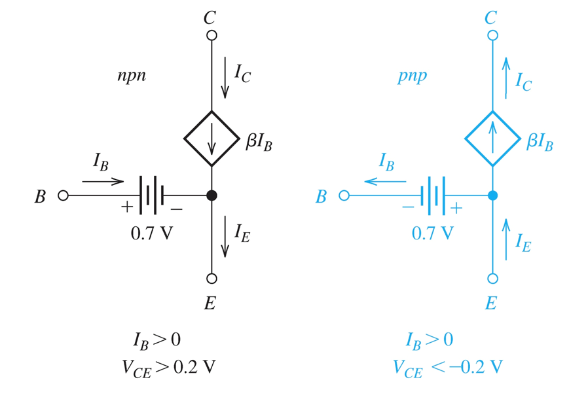
\includegraphics[width = .5\textwidth]{LSMforward.png}   
    
    One Diode On
\end{center}
\subsubsection*{Saturation}
\begin{center}
    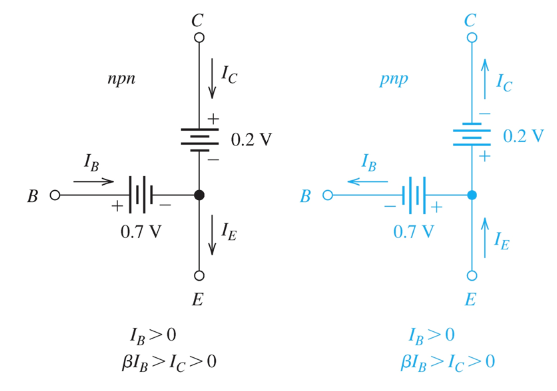
\includegraphics[width = .5\textwidth]{LSMsaturation.png}   
    
    Both Diodes On
\end{center}
\subsubsection*{Cutoff}
\begin{center}
    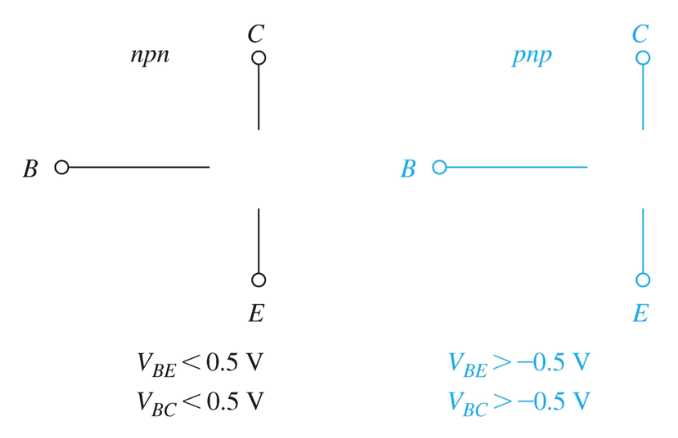
\includegraphics[width = .5\textwidth]{LSMcutoff.png}
    
    Both Diodes Off
\end{center}
\subsection*{Four Resistor Bias Networks}
\begin{center}
    Relatively independent of beta value allowing for temperature fluctuations and a common use of the forward active region of operation.

    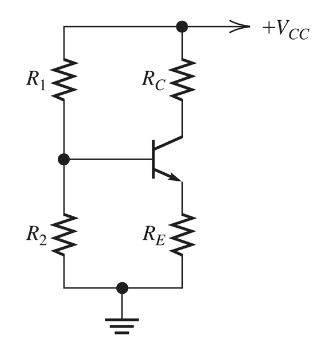
\includegraphics[width = .2\textwidth]{FRBnetwork.png}
    
    To calculate the equivalent for the left side of the network:
\end{center}
\begin{equation}
    V_{BB} = V_{CC} \frac{R_2}{R_1+R_2}
\end{equation}
\begin{equation}
    R_{BB} =  R_1 \parallel R_2
\end{equation}
\begin{center}
    To calculate the Quiescent point:
\end{center}
\begin{equation}
    I_B = \frac{V_{BB} - V_{BE}}{R_{BB} + (\beta +1) R_E}
\end{equation}
\begin{equation}
    I_C = \beta I_B
\end{equation}
\begin{equation}
    V_{CE} = V_{CC} - I_C (R_C + R_E)
\end{equation}
\subsection*{Rectifiers}
\subsubsection*{Notation}
\begin{equation}
    Q \cong I_L T
\end{equation}
\begin{equation}
    V_r = \frac{Q}{C}
\end{equation} 
\begin{equation}
    V_L = V_m - \frac{V_r}{2}
\end{equation}
\begin{center}
    $Q$ is the \textbf{charge loss}
    
    $I_L$ is the \textbf{load current}
    
    $T$ is the \textbf{period}
    
    $V_r$ is the \textbf{ripple voltage}
    
    $V_m$ is the \textbf{max voltage}
    
    $V_L$ is the \textbf{average DC voltage}
\end{center}
\subsubsection*{Half-wave}
\begin{center}
    The peak inverse voltage is a design consideration because if it surpasses the diode breakdown then it will damage the diode and is therefore a design consideration.
    \vspace{3mm}
    
    PIV $= -2V_m$
\end{center}
\begin{equation}
    C = \frac{I_L T}{V_r}
\end{equation}
\subsubsection*{Full-wave}
\begin{center}
    In the full wave rectifier the peak inverse voltage is defined as follows:
\end{center}
\begin{equation}
    PIV \cong V_m
\end{equation}
\begin{equation}
    C = \frac{I_L T}{2 V_r}
\end{equation}
\begin{center}
    The full wave rectifier produces less ripple for the same amount of cap and has less PIV and is therefore the industry standard.
\end{center}
\vspace{8mm}
\subsection*{Small Signal Model for BJTs}
\newpage
% Exam 3 ===================================
% Exam 4 ===================================
\section*{Exam Four}
\begin{center}
    haha i am very lazy sorry
\end{center}
% Exam 4 ===================================
\end{document}
